\subsection{Diseño del Amperímetro de tres rangos}
En esta sección se describen los cálculos realizados para determinar las resistencias de calibración (\( R_c \)) y las resistencias shunt (\( R_{sh} \)) correspondientes a cada rango de medición del amperímetro. Para ello, se utilizó un código en MATLAB que por la facilidad de adaptar los valores de \( R_{sh} \) y \( R_c \) de acuerdo con nuevos requerimientos o con modificaciones sobre la marcha en los valores de la resistencia interna del galvanómetro (\( R_g \)) o de los rangos deseados.

El amperímetro fue diseñado para medir en tres rangos de corriente: 10 mA, 50 mA y 100 mA. Para ello, se fijó una sensibilidad de 700 \(\Omega/V\), lo que implica que la corriente máxima que podría medir el galvanómetro es \( I_m = \frac{1}{s} \), donde \( s \) es la sensibilidad en \(\Omega/V\), la cual debe ser corregida mediante la incorporación de la resistencia de calibración para llevar la corriente máxima al valor aceptado por el galvanómetro de correspondiente a 1 [mA]. 

El cálculo de la resistencia shunt para cada rango de corriente se realizó utilizando la fórmula \ref{eq:Rsh} descrita en el marco teórico, donde \( R_g = 391 \, \Omega \) es la resistencia interna del galvanómetro e \( I_{\text{rango}} \) es la corriente máxima para cada rango.

Del mismo modo, se calcula el valor de la resistencia de calibración necesaria para cada rango a partir de lo expuesto en el marco teórico, junto con determinar el valor que permite un ajuste de +-10\% en la corriente que pasa por el galvanómetro. 

A continuación, se presentan los resultados obtenidos para las resistencias de calibración \( R_c \) y las resistencias shunt \( R_{sh} \) para cada rango de corriente:

\begin{table}[h]
\centering
\caption{Resultados de las resistencias de calibración y shunt para cada rango de corriente.}
\begin{tabular}{|c|c|c|c|c|}
\hline
\textbf{Rango} & \textbf{\( R_{sh} \) [Ohm]}  & \textbf{\( R_c \) [Ohm]} & \textbf{\( R_c \) +10\% [Ohm]} & \textbf{\( R_c \) -10\% [Ohm]} \\ \hline
\textbf{10 mA}  & 65.17 & 195.5 & 260.67 & 130.33 \\ \hline
\textbf{50 mA}  & 11.5 & 172.5  & 230.0  & 115.0  \\ \hline
\textbf{100 mA}  & 5.67 & 170.0 & 226.67 & 113.33 \\ \hline
\end{tabular}
\label{tab:ResitShuntyCal}
\end{table}


\subsection{Simulación}
Para verificar la validez de los cálculos realizados y asegurarse de que el diseño del amperímetro funcione correctamente en los tres rangos, se modeló el sistema en el software de simulación PLECS. En este modelo, se replicó el funcionamiento del galvanómetro y se observaron los resultados en función de las resistencias shunt (\( R_{sh} \)) conectadas en paralelo con el galvanómetro.

El modelo simulado incluye los tres rangos de medición (10 mA, 50 mA y 100 mA), cada uno de los cuales depende de los valores de \( R_{sh} \), ajustados previamente en los cálculos. El diagrama de simulación muestra cómo se conecta el selector de rangos y cómo las resistencias shunt permiten el funcionamiento adecuado del amperímetro a diferentes niveles de corriente.

A continuación se presenta la imagen del circuito simulado en PLECS:

\begin{figure}[h]
    \centering
    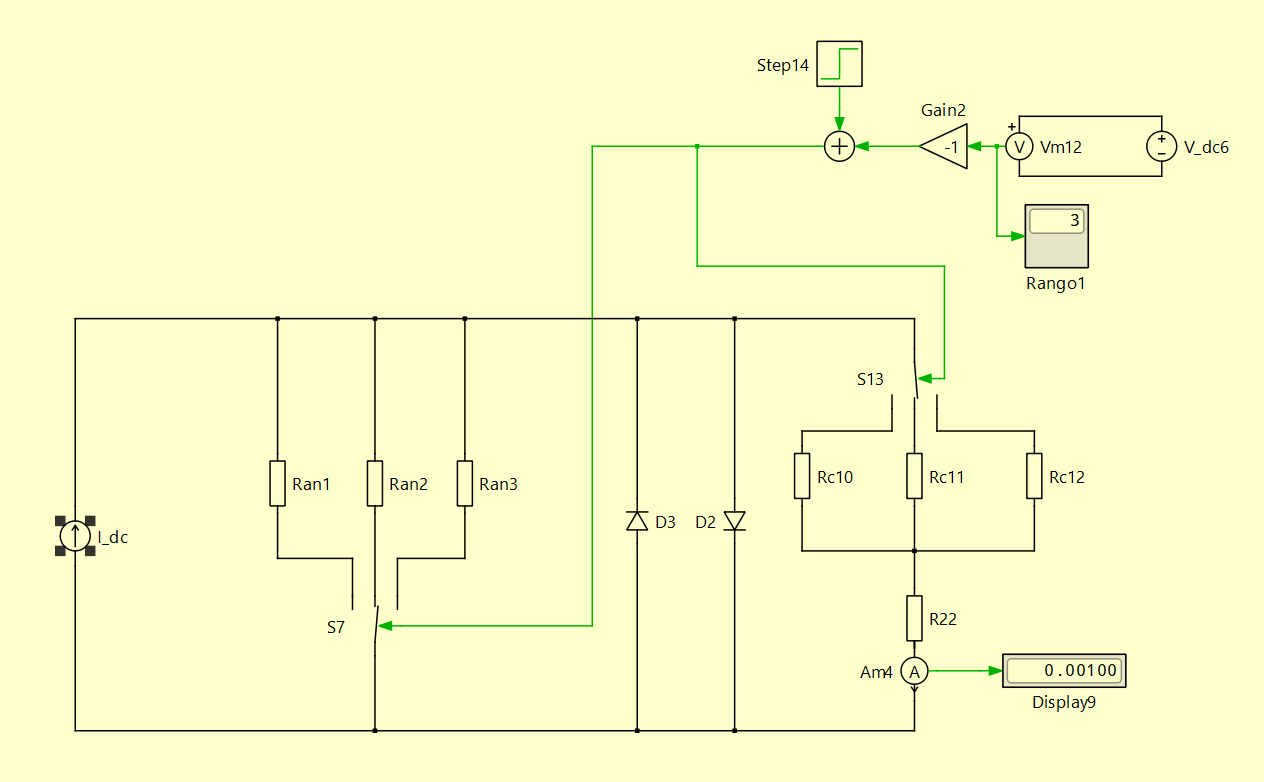
\includegraphics[width=0.7\textwidth]{recursos/imagen_2025-10-22_013807311.png}
    \caption{Modelo del amperímetro en PLECS con tres rangos de corriente dependientes de las resistencias shunt.}
\end{figure}

La simulación mostró que el amperímetro responde correctamente según lo esperado, y los resultados coinciden con los cálculos previos. En cada rango, la corriente medida por el galvanómetro se ajusta adecuadamente, garantizando que las deflexiones de la aguja correspondan a las corrientes máximas especificadas para cada rango de medición.

El ajuste de las resistencias shunt en paralelo con el galvanómetro en la simulación permitió corroborar que el sistema funciona correctamente y que los cálculos realizados para \( R_{sh} \) y \( R_c \) están en línea con el comportamiento teórico del amperímetro.

% --- INICIO DEL CÓDIGO PARA AGREGAR ---


\subsection{Construcción de Resistencias Shunt con Nicrom}
\label{sec:nicrom}

Como parte del trabajo previo, se debe calcular la implementación física de las resistencias shunt ($R_{sh}$). Se sugiere la construcción de estos shunts utilizando alambre de Nicrom, calculando la longitud necesaria del mismo.

Para los cálculos siguientes, se considera un alambre de Nicrom disponible en el pañol, el cual se encuentra rotulado con una resistencia lineal ($\rho_L$) de 5.8 $\Omega$/metro.

La longitud ($L$) requerida para cada resistencia se obtiene dividiendo el valor de resistencia shunt deseado ($R_{sh}$) por la resistividad lineal del alambre ($\rho_L$):
$$ L = \frac{R_{sh}}{\rho_L} $$

Aplicando esta fórmula a los valores de $R_{sh}$ calculados en la Tabla \ref{tab:ResitShuntyCal} (ver sección 4.1), se obtienen las siguientes longitudes de alambre:

\begin{itemize}
    \item \textbf{Rango 1 (10 mA):} Se requiere una $R_{sh1} = 65.16~\Omega$.
        $$ L_1 = \frac{65.16~\Omega}{5.8~\Omega/m} = 11.23~\text{m}$$

    \item \textbf{Rango 2 (50 mA):} Se requiere una $R_{sh2} = 11.5~\Omega$.
        $$ L_2 = \frac{11.5~\Omega}{5.8~\Omega/m} = 1.98~\text{m}$$

    \item \textbf{Rango 3 (100 mA):} Se requiere una $R_{sh3} = 5.66~\Omega$.
        $$ L_3 = \frac{5.66~\Omega}{5.8~\Omega/m} = 0.97~\text{m}$$
\end{itemize}

\newpage
\subsection{Diseño del Circuito de Contrastación}
\label{sec:contrastacion}

Finalmente, la guía solicita diseñar el circuito de contrastación para el instrumento. Para el caso del amperímetro, este circuito debe permitir generar las corrientes de fondo de escala (10 mA, 50 mA y 100 mA) de forma controlada. A diferencia de un método tradicional, en esta experiencia se utilizó una fuente electrónica de tensión de $10~V_{cc}$ variable y solo una resistencia limitadora fija $R_{lim}$ para cada rango, omitiendo el uso de potenciómetros. La variación para obtener los puntos de linealidad se logra ajustando el voltaje de la fuente desde 10 V hacia abajo. El esquema base de este circuito se presenta en la Figura \ref{fig:circuito_prueba_amperimetro}.

\begin{figure}[h!]
  \centering
  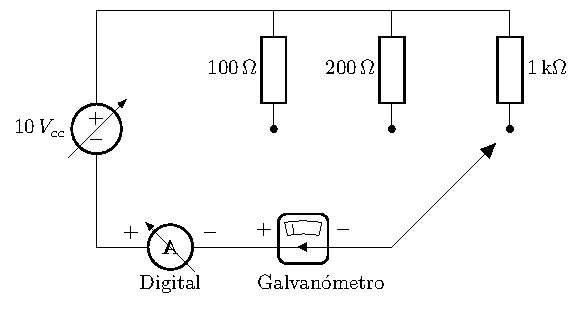
\includegraphics[width=0.7\linewidth]{recursos/circuito_contrastacion.pdf}
    \caption{Esquema del circuito de prueba para la calibración y contrastación del amperímetro empleando resistencia limitadora fija.}
    \label{fig:circuito_prueba_amperimetro}
\end{figure}

Para el cálculo de la resistencia limitadora total ($R_{\text{lim}}$) necesaria para cada rango, se utiliza la Ley de Ohm. Se asume la fuente ajustada a $10~V_{cc}$ y se desprecia la resistencia interna del amperímetro para simplificar la selección de los componentes fijos.

$$ R_{\text{lim}} = \frac{V_{cc}}{I_{\text{rango}}} $$

Los valores de resistencia fija necesarios para alcanzar la corriente de fondo de escala en cada rango a 10 V se resumen en la Tabla \ref{tab:res_prueba}. En la práctica, se implementará esta $R_{\text{lim}}$ mediante una resistencia fija de valor cercano al estándar comercial.

\begin{table}[h!]
    \centering
    \caption{Cálculo de resistencias limitadoras totales para el circuito de prueba con $V_{cc} = 10~V$.}
    \label{tab:res_prueba}
    \begin{tabular}{cccr}
        \toprule
        \textbf{Rango} & \textbf{Rango ($I_{\text{rango}}$)} & \textbf{Fuente ($V_{cc}$)} & \textbf{Resistencia ($R_{\text{lim}}$)} \\
        \midrule
        1 & 10 mA & 10 V & $R_{\text{lim1}} = \frac{10~V}{10~mA} = \mathbf{1~k\Omega}$ \\
        2 & 50 mA & 10 V & $R_{\text{lim2}} = \frac{10~V}{50~mA} = \mathbf{200~\Omega}$ \\
        3 & 100 mA & 10 V & $R_{\text{lim3}} = \frac{10~V}{100~mA} = \mathbf{100~\Omega}$ \\
        \bottomrule
    \end{tabular}
\end{table}

\newpage
\subsection{Diseño del Circuito de Carga en Paralelo}
\label{sec:paralelo}

Adicionalmente, se solicita en la guía de la experiencia (punto 2.4.g) la aplicación de $10~V_{cc}$ a tres resistores en paralelo, para medir tanto la corriente de cada resistor como la corriente de la fuente, utilizando los rangos apropiados del amperímetro construido.

Para esto, se diseñó un circuito de carga como el mostrado en la Figura \ref{fig:circuito_paralelo}, alimentado por una fuente $V_{cc}$ de 10 V. El objetivo es que la corriente total ($I_{\text{fuente}}$) sea de 100 mA, correspondiente al rango máximo del instrumento, y que las corrientes individuales ($I_1$, $I_2$, $I_3$) se distribuyan de forma que puedan medirse con los distintos rangos (100 mA, 50 mA y 10 mA).

\begin{figure}[h!]
  \centering
  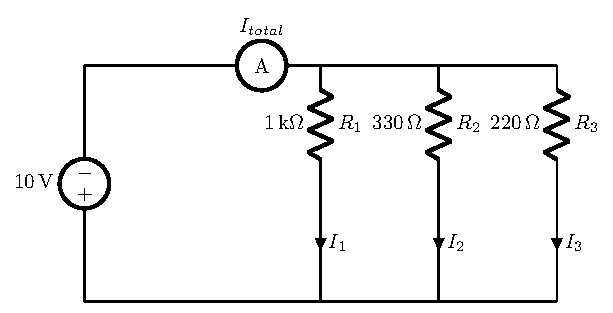
\includegraphics[width=0.7\linewidth]{recursos/circuito_validacion.pdf}
    \caption{Esquema del circuito de prueba con carga en paralelo.}
    \label{fig:circuito_paralelo}
\end{figure}

Se buscaron valores de resistencia comerciales que, asumiendo una tensión ideal de 10 V en sus terminales, generaran las corrientes deseadas dentro de los rangos del instrumento. Los valores seleccionados se resumen en la Tabla \ref{tab:res_paralelo}.

\begin{table}[h!]
    \centering
    \caption{Resistencias de carga en paralelo y corrientes teóricas.}
    \label{tab:res_paralelo}
    \begin{tabular}{cccl}
        \toprule
        \textbf{Componente} & \textbf{Corriente teórica $I_n$} & \textbf{Resistencia seleccionada $R_n$} & \textbf{Rango a Utilizar} \\
        \midrule
        $R_1$ & 10 mA & 1 k$\Omega$ & 10 mA \\
        $R_2$ & 30.3 mA & 330 $\Omega$ & 50 mA \\
        $R_3$ & 45.4 mA & 220 $\Omega$ & 50 mA \\
        \midrule
        Total & $\sim$ 85.7 mA & - & 100 mA \\
        \bottomrule
    \end{tabular}
\end{table}

\newpage
Según el diseño, la corriente total que debe entregar la fuente es la suma de las corrientes individuales:
$$ I_{\text{fuente}} = I_1 + I_2 + I_3 = 10~\text{mA} + 30.3~\text{mA} + 45.4~\text{mA} \approx 85.7~\text{mA} $$
Este valor es inferior a los 100 mA del rango máximo del amperímetro, garantizando una validación segura del instrumento sin riesgo de sobrecorriente.